% !TeX root = ../main.tex
% Add the above to each chapter to make compiling the PDF easier in some editors.

\chapter{Related Work}\label{chapter:relWork}

\textit{Should the related work section be put AFTER the eSIM Architecture section? The content of related papers is easier to understand, when terms and concepts are already known.}

This chapter summarizes the related work on both the topics security analysis of eSIM and further or proposed improvements and unification of the two standards.

\section{Security Analysis of eSIM}
The security analysis of both the M2M and Consumer \acrshort{eUICC} Architecture is a big part of this thesis. So far, however, little research has been published on the security of the eSIM.

The GSMA itself provides a Common Criteria Protection Profile (\acrshort{PP}) for both \acrshort{M2M} (SGP.05 \parencite{SGP:05}) and Consumer (SGP.25 \parencite{SGP:25}) for certification of the eUICC against EAL4. The PPs of course note the differences between the two standards, but are very similar to each other in analysis strategy and approach, which is why the following summary is relevant to both. The "Target of Evaluation" (TOE) of both protection profiles is the software, that implements the GSMA Remote Provisioning Architecture within the eUICC. More precisely, it includes two layers. The fist being the application layer to implement the \acrshort{RSP} functionalities, comprising of ISD-P and ISD-R, ECASD and MNO-SD. The second is the platform layer, which consists of a telecom framework to access mobile networks, a profile package interpreter that translates profile package data into the internal eUICC profile format, and a profile policy enabler. The PP then lists several security assets for each layer, e.g. User Data, Profile Data etc.. These assets need protection in terms of Confidentiality, Integrity and Availability (CIA) which results in a list of threats (e.g. Unauthorized Profile Management, Interception etc.). The extensive document then proposes requirements for the security of the system, but does not scrutinize how that security is implemented.

Ding et al. have published two different papers focusing on the M2M eSIM Session Key Agreement Protocol \parencite{Ding:SecAnalySPIN} \parencite{Ding:FormAnalSessionKey}. The Key Agreement is used to create a symmetric \acrshort{AES} key for securing any further communication between the provisioning server (SM-DP) and eUICC (ISD-P). It is explained in more detail in section \ref{chapter:eSIMArch} as it precedes and is relevant for the profile download. The authors use model testing to formally analyze the session key creation process. In \parencite{Ding:SecAnalySPIN}, this process is simplified to three interactions between SM-DP and eSIM (random challenge by eUICC, encrypted response from SM-DP, shared secret from eUICC). The attacker against the model is built according to the Dolev-Yao Attacker \parencite{Dolev:Yao}, which can always intercept, modify, replay or store any messages between the targets.
In \parencite{Ding:FormAnalSessionKey}, Petri Nets are used to model the session key agreement in more detail.
In both papers, the respective model is formally analyzed using the model verification tool SPIN \parencite{SPIN}. The papers report a secure session key agreement protocol without any dead- or livelocks during operation, since the attacker needs to obtain the key in order to be able to decrypt any messages.

Zhao et al. \parencite{Zhao:SecureSIM} are investigating the PIN-based access control to \acrshort{SIM} functionalities and stored data. Modems (and in consequence end users) are required to enter a PIN at most once after the boot procedure to be able to use all SIM features correctly. There is no authorization control afterwards. This directly translates to eSIM, as the mechanism is re-used in the new version. The authors survey users and report that most do not use a SIM PIN at all, which even increases the feasibility of their devised attacks (one-time access, traffic eavesdropping, Man in the middle and impersonation) against user data and network communication. They propose a "SecureSIM", which implements more fine grained access control via an access graph and certificate based authorization between (e)SIM and modem.

Ahmed et al. \parencite{Ahmed:TransparancyProfile} questions the trust placed into the PKI of the consumer RSP architecture, since all parties automatically trust all other parties that are certified by the GSMA CI.
The authors' argument is that while the system is secure against outside attackers, it is compromised if one server (e.g. SM-DP+) gets breached, since this server is able to clone and provision profiles to blindly trusting eUICCs, resulting in business loss for the MNO of the target profile. As a solution, they propse a "SIM profile transparency protocol (SPTP)", which allows MNOs to keep track of provisioned IMSIs and registers IMSIs bound to the respective EID in a transparency ledger. 
The new protocol is formally analyzed using ProVerif with the goals being, that "an eUICC only accepts a profile from a server if and only if there exists a unique binding for the profile in the ledger" and "an MNO can detect any mis-issuance or clone of a profile" \parencite{Ahmed:TransparancyProfile}. Both goals are achieved for so-called honest and dishonest servers. A server is dishonest, if it is trusted by the GSMA CI, but performs malicious or undesired operations.

Lastly, a few practical attacking possibilities have been shown for an earlier version of the M2M specification \parencite{SGP:02v3} by Meyer et al. \parencite{Meyer:AttackseSIM} with a focus on memory exhaustion and profile policy rules: 
\begin{itemize}
    \item A network adversary could launch a memory exhaustion attack against an eUICC by dropping response messages to the SM-SR after ISD-P creation. This would lead to the SM-SR asking again for ISD-P creation until the internal eUICC memory is full.
    \item A malicious SM-SR could send an under-representation of the remaining eUICC memory to the SM-DP on request. The SM-DP is then unable to install a new profile since the eUICC memory is considered full.
    \item A malicious MNO could request a bloated profile to be installed on the eUICC, instantly filling the target memory.
    \item A malicious MNO can install profiles with the profile policy rule "CannotBeDisabled" either to true or false and lock the device.
\end{itemize}
The findings of \parencite{Meyer:AttackseSIM} have been reported to the GSMA and a fix for the memory exhaustion attack was implemented in the next version (v3.2). The authors however also state, that more issues may still exist and further investigation on the standard is necessary.

Since a direct assessment of the whole eSIM architecture was not published to date, security analyses of comparable systems should also be reviewed. One structure in the IoT ecosystem looks promising and offers a larger range of related work: Firmware over the air updates (FotA).

In FotA, the software of a device is updated over a wireless connection like Wi-Fi or mobile networks. In the IoT it often needs an option to deploy (almost) the same software to multiple devices at once in a secure fashion, which can be compared to provisioning a new eSIM-Profile, with the difference being, that the profile is individual for every eUICC.

Zandberg et al. \parencite{Zandberg:SecFirmwareUpdatesforIoT} survey existing open FotA standards and design a prototype for IoT firmware updates based on these standards. They classify the FotA system into three work areas: Embedded Software design to enable updates on the target platform, a backend framework to compile the image and a network transport area to provision the images to the target device. SUIT (software updates for internet of things) is a promising framework by the IETF and one possible configuration of their prototype. The authors test this prototype against eight different threats: Tampered firmware, firmware replay, offline device attack, firmware mismatch, flash memory location mismatch, unexpected precursor image, reverse engineering and resource exhaustion. The SUIT manifest already implements many mitigation strategies. Finally, they conclude their paper with experiments on the performance of different cryptographic algorithms and FotA configurations. State-of-the-art security is in their opinion doable even on resource constrained IoT devices, but real world requirements, such as firmware encryption, version management and time-to-market often make firmware updates a complex task.

In \parencite{Dejon:AutomatedSecurityAnalysisofFotA}, Dejon et al. also see the eight threat categories found by \parencite{Zandberg:SecFirmwareUpdatesforIoT} targeting the integrity and confidentiality of the update process. These threats should in their opinion be directly handled by an appropriate implementation of SUIT. The authors see a bigger risk in SUIT assuming a trusted and reliable input image and therefore propose an IoT Application verification framework (IoTAV) to additionally assess the security of the IoT application before provisioning it. The security evaluation of this image relies on inter-procedural control flow graphs to automatically model the specific software and check it against Linear Temporal Logic Formulas.

% FotA Updates could also be applied to the devices in Wireless Sensor Networks. On the other hand, WSNs are already an interesting system and comparable to the eSIM architecture, as many nodes and devices with various roles and permissions communicate with each other - often authenticated though a central PKI.

\section{Developments on the eSIM Concept}

The second part of this work focuses on further improving the two standards and merging one into another, such that one system allows for a push and pull of a profile with the same hardware and architecture. Such a notion has never been proposed before, however, there exist some ideas for a further enhancement of the specifications.


\begin{figure}[ht]
    \centering
    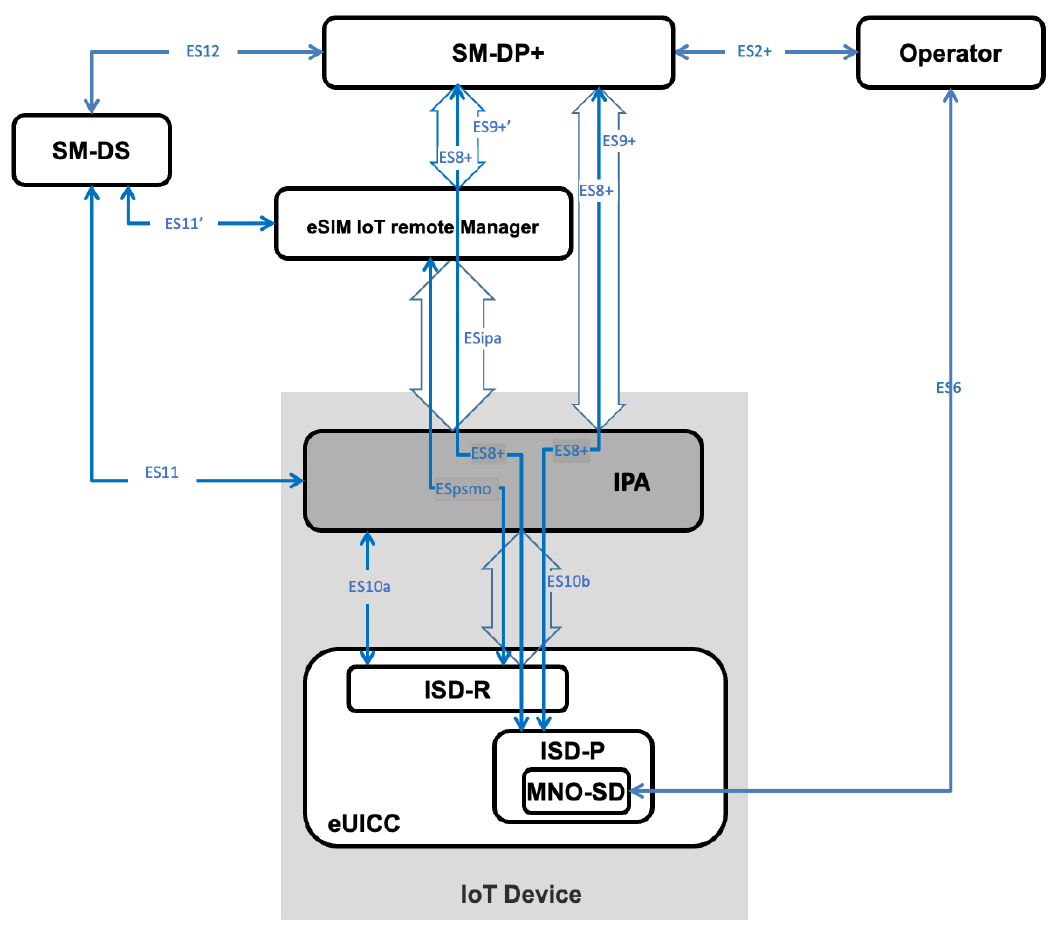
\includegraphics[width=0.65\textwidth]{pictures/iot_architecture.png}
    \caption{GSMA IoT (SGP.31) Architecture \parencite{SGP:31}}
    \label{fig:iot_arch}
\end{figure}
In April 2022, the GSMA has published a third eSIM specification class: The eSIM architecture for the Internet of Things \parencite{SGP:31}. It is based on the Consumer Architecture and adds an eSIM IoT remote Manager for remote Profile State Management of single or multiple IoT devices. In essence, the IoT Remote Manager provides a profile download triggering message (containing Activation Code, SM-DP+ Address or SM-DS event) to the IoT Profile Assistant (IPA). The IPA then acts similar to the Consumer LPA to download the profile. Therefore, a profile push can be managed via the existing pull mechanisms. A more in-depth description will be in chapter \ref{chapter:merging}, as the proposed merger will be compared to the GSMA IoT Specification. The GSMA however does not see the SGP.31 as a unification of M2M and Consumer, but rather as a new architecture to provision profiles to resource constrained, IoT devices. Additionally, only the architecture has so far been released. A detailed technical specification explaining the used protocols and interfaces is expected at the end of 2022.

As already mentioned, Zhao et al. \parencite{Zhao:SecureSIM} and Ahmed et al. \parencite{Ahmed:TransparancyProfile} propose extensions to the eSIM architecture in their analysis of the system. Lv et al. \parencite{Lv:NbIoTeSIM} want to use eSIMs in Narrowband-IoT (NB-IoT) networks. Since NB-IoT is a very constrained network with terminals being the bottleneck for profile provisioning, they try a smarter load balancing strategy by assigning terminals a fixed priority and relay. The reliability and system performance is analyzed using Markov Chains. In their simulation, throughput and outage probability of their system performs much better.

This master thesis will perform the first holistic external security analysis on the two remote provisioning eSIM architectures (M2M and consumer). Based on the vulnerabilities found, solution approaches will then be presented and a new architecture will be proposed to cover the requirements of both specifications.